\section{Conclusion}
The most accurate predictive model that I created was the Random Forest Classifier with a 93\%. \cref{fig:rf_features} shows the most significant feature weights that the model iteratively learned.

\begin{figure}[H]
    \centering
    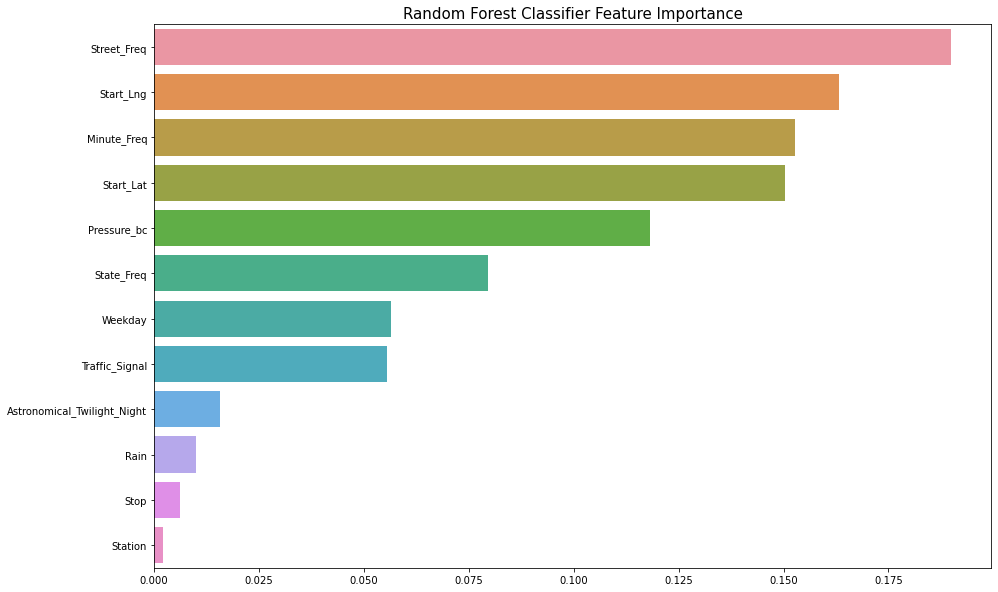
\includegraphics[width=130mm,height=\textheight,keepaspectratio]{images/rf_features.png}
    \caption{Random Forest Classifier Feature Importance}
    \label{fig:rf_features}
\end{figure}

\noindent
The 5 most important features it determined were:
\begin{enumerate}
    \item Street Frequency
    \item Start Longitude
    \item Minute Frequency
    \item Start Latitude
    \item Pressure (Box-Cox)
\end{enumerate}

I am not surprised that Street Frequency, Start Longitude, and Start Latitude were in the top 5. As seen in \cref{section:exploratory_analysis}, most severe accidents seemed to occur on interstate highways in densely populated regions (based on longitude and latitude). Along with the temporal input that the Minute Frequency feature provided, the pattern clearly indicates that severe accidents are likely to occur in the same location and time as severe accidents that have occurred in the past.

Unlike the other factors, I was surprised by the Pressure (Box-Cox) feature being so important. Since a strong negative correlation was found for this factor, I wonder if pressure plays an indirect role in causing severe accidents. This is unlikely to be due to the weather as none of the weather features like Rain seemed to have a strong correlation with severity. 

I was also surprised to see factors like Astronomical Twilight Night and Traffic Signal to only be somewhat important in predicting severe accidents as these are often cited as common dangerous driving conditions. As a further exploration, I would like to investigate these anomalies.